\ifx \globalmark \undefined %% This is default.
	\documentclass[a4paper,12pt]{report}

%%% PACKAGES %%%

\usepackage[french, english] {babel}	% langue principale
\usepackage[ansinew]{inputenc}
\usepackage[T1]{fontenc}		% Police contenant les caractères français
\usepackage{lmodern}			% plus beau
\usepackage[a4paper]{geometry}
	\geometry{hscale=0.75,vscale=0.8,centering}

\usepackage[hidelinks]{hyperref} % pas de couleurs ici
%
\usepackage[natbibapa]{apacite}

%% Maths
\usepackage{amsfonts} % Equations etc
\usepackage{amsmath}
\usepackage{mathtools}
\usepackage{amssymb}

\usepackage{cleveref}

%% Itemizes
\usepackage{enumerate}
\usepackage{enumitem}

%% Dessins & Plots
\usepackage[pdftex]{graphicx} %Images dans le PDF
\usepackage{epstopdf}
\usepackage{color, xcolor}
%% Dates
\usepackage{datetime}
\newdateformat{monthyeardate}{\monthname[\THEMONTH] \THEYEAR}
\usepackage{chessboard}
\usepackage{booktabs,tabularx,multirow}
\usepackage[babel=true,kerning=true]{microtype}
%> Tikz
\usepackage{tikz}
\usepackage{hf-tikz}
\usetikzlibrary{
	calc,
	arrows,
	arrows.meta,
	automata,
	shapes,
	snakes,
	positioning,
	decorations,
	decorations.text,
	fit,
	matrix,
	mindmap
	}
	\tikzstyle{noeud-std}=[draw,fill=black,circle,inner sep=0pt,minimum size=7pt]% 7pt est la taille des cercles noirs
\usepackage{tkz-graph}
\newcommand{\tikzmark}[2]{\tikz[overlay,remember picture,baseline=(#1.base)] \node (#1) {#2};}
\newcommand{\Highlight}[1][submatrix]{%
    \tikz[overlay,remember picture]{
    \node[highlight,fit=(left.north west) (right.south east)] (#1) {};}
    }
\tikzset{%
  highlight/.style={rectangle,rounded corners,fill=ocre!50,draw,
    fill opacity=0.5,thick,inner sep=0pt}
}
\newcommand{\mytikzmark}[2]{\tikz[overlay,remember picture, baseline=(#1.base)] \node (#1) {#2};}


%% Meta
\usepackage{etoolbox}

% Debugging purposes: Catch when a reference is missing
\makeatletter
	\patchcmd{\@setref}{\bfseries ??}{{\color{red}[\texttt{\detokenize{ #3 }}]}}{}{%
	  \GenericWarning{}{Failed to patch \protect\@setref}}
	\patchcmd{\@citex}{\bfseries ?}{{\color{red}[\texttt{\detokenize{ #3 }}]}}{}{%{{\color{red}\texttt{\@citeb}}}{}{%
	  \GenericWarning{}{Failed to patch \protect\@citex}}
\makeatother

%% CUSTOM ENVIRONMENTS
% Packages
\usepackage{framed}
\usepackage{mdframed}
\usepackage[amsmath,thref, framed]{ntheorem}

%% Counters for theorem.
% The current choice is that all environments share a counter within chapters.
% It that regards, it becomes easy to navigate the document.

\newcounter{theo}[chapter]\setcounter{theo}{0}
\renewcommand{\thetheo}{\arabic{chapter}.\arabic{theo}}



% The following is adapted from https://texblog.org/2015/09/30/fancy-boxes-for-theorem-lemma-and-proof-with-mdframed/
% \newenvironment{name}[args]{begin_def}{end_def}
\newenvironment{generic_theo}[2][] % 2 arguments, and one is optional. The first argument will say if we have a Thm or somth, the second is the name of the thm.
	{% begin_def
		\refstepcounter{theo}%
		\ifstrempty{#2} % looking at the name of the thm
		{
			\mdfsetup{
				frametitle={
					\tikz[baseline=(current bounding box.east),outer sep=0pt]
					\node[anchor=east,rectangle,fill=white!20, draw = black!20, line width = 2pt]
					{\strut #1~\thetheo};}
			} % The #1 will say Theorem, or other.
		}
		{
			\mdfsetup{
				frametitle={
				\tikz[baseline=(current bounding box.east),outer sep=0pt]
				\node[anchor=east,rectangle,fill=white!20, draw = black!20, line width = 2pt]
				{\strut #1~\thetheo:~#2};}
			}
		}
		\mdfsetup{innertopmargin=10pt,linecolor=black!20,
					linewidth=2pt,topline=true,
					frametitleaboveskip=\dimexpr-\ht\strutbox\relax
				}
\begin{mdframed}[]\relax}{\end{mdframed}}


%% Proofs (slightly different)
\newenvironment{generic_proof}[2][] % 2 arguments, and one is optional. The first argument will say if we have a Thm or somth, the second is the name of the thm.
	{% begin_def
		\refstepcounter{theo}%
		\ifstrempty{#2} % looking at the name of the thm
		{
			\mdfsetup{
				frametitle={
					\tikz[baseline=(current bounding box.east),outer sep=0pt]
					\node[anchor=east,rectangle,fill=black!20]
					{\strut #1~\thetheo};}} % The #1 will say Theorem, or other.
		}
		{
			\mdfsetup{
				frametitle={
				\tikz[baseline=(current bounding box.east),outer sep=0pt]
				\node[anchor=east,rectangle,fill=black!20]
				{\strut #1~\thetheo:~#2};}}
		}
		\mdfsetup{innertopmargin=10pt,linecolor=black!20,
					linewidth=1pt,topline=true,
					frametitleaboveskip=\dimexpr-\ht\strutbox\relax
				}
\begin{mdframed}[]
}{\end{mdframed}}

%% Examples/Exercices
\newenvironment{generic_ex}[2][] % 2 arguments, and one is optional. The first argument will say if we have a Thm or somth, the second is the name of the thm.
	{% begin_def
		\refstepcounter{theo}%
		\ifstrempty{#2} % looking at the name of the thm
		{
			\mdfsetup{
				frametitle={
					\tikz[baseline=(current bounding box.east),outer sep=0pt]
					\node[anchor=east,rectangle,fill=black!20]
					{\strut #1~\thetheo};}} % The #1 will say Theorem, or other.
		}
		{
			\mdfsetup{
				frametitle={
				\tikz[baseline=(current bounding box.east),outer sep=0pt]
				\node[anchor=east,rectangle,fill=black!20]
				{\strut #1~\thetheo:~#2};}}
		}
		\mdfsetup{innertopmargin=10pt,linecolor=black!20,
					linewidth=1pt,topline=true,
					frametitleaboveskip=\dimexpr-\ht\strutbox\relax
				}
\begin{mdframed}[]
}{\end{mdframed}}



% The different environments that we need (Main stuff are highlighted.
\newenvironment{theorem}[1][]{\begin{generic_theo}[Theorem]{#1}}{\end{generic_theo}}
\newenvironment{lemma}[1][]{\begin{generic_theo}[Lemma]{#1}}{\end{generic_theo}}
\newenvironment{definition}[1][]{\begin{generic_theo}[Definition]{#1}}{\end{generic_theo}}
\newenvironment{notation}[1][]{\begin{generic_theo}[Notation]{#1}}{\end{generic_theo}}
\newenvironment{proposition}[1][]{\begin{generic_theo}[Proposition]{#1}}{\end{generic_theo}}
\newenvironment{procedure}[1][]{\begin{generic_theo}[Procedure]{#1}}{\end{generic_theo}}
\newenvironment{hypothese}[1][]{\begin{generic_theo}[Hypothesis]{#1}}{\end{generic_theo}}


% These ones, let's not overblow them
% The true reason why I'm doing this is that there may be floats in Exercices and Examples...
% You can't have  begin{figures} in mdframed env, it crashes.
%\newtheorem{notation}[theo]{Notation}
\newcounter{axiomc}[chapter]\setcounter{axiomc}{0}
\renewcommand{\theaxiomc}{\arabic{chapter}.\arabic{axiomc}}

\newtheorem{axiom}[axiomc]{Axiom}
\newtheorem{proof}[theo]{Proof}
\newtheorem{exercise}[theo]{Exercise}
\newtheorem{example}[theo]{Example}



%% CUSTOM Commands

% Identify TAs
\newcommand{\TAone}{Mahsa}
\newcommand{\TAtwo}{Beno\^it}

\newcommand{\reels}{\mathbb{R}}

\DeclareMathOperator*{\argmin}{arg\,min}
\DeclareMathOperator*{\argmax}{arg\,max}

% Nice brackets
\newcommand\parent[1]{\left(#1\right)}
\newcommand\abs[1]{\left\lvert#1\right\rvert}
\newcommand\norm[1]{\left\lVert#1\right\rVert}
\newcommand\bracket[1]{\left\{#1\right\}}
\newcommand\squared[1]{\left[#1\right]}

\DeclarePairedDelimiter{\floor}{\lfloor}{\rfloor}
\DeclarePairedDelimiter{\ceil}{\lceil}{\rceil}
\usepackage{eurosym}
\usepackage{siunitx}
\DeclareSIUnit{\EUR}{\text{\euro}}
\sisetup{
  per-mode = fraction,
  inter-unit-product = \ensuremath{{}\cdot{}},
}



\usepackage{textcomp}
\let\texteuro\euro





	\begin{document} %% Crashes if put after (one of the many mysteries of LaTeX?).	
\else 	
\fi




\chapter{The Nash Equilibrium} \label{chap:Nash}
{\large{\itshape
``People usually call them Nash equilibria, but I just call them equilibria.''} --- John Nash (1928 -- 2015).\\
}
{\small{\itshape
Chapter based on pages 91-108 and 122-127 of the book  ``Game theory - Analysis of conflict'' by R. Myerson.}\\
}


The utility maximization theorem of the first chapter \emph{quantifies} the behaviour 
of a rational and intelligent agent, having to make decisions in an uncertain environment. 
We can always expect an agent to perceive the uncertainties through a \emph{conditional probability function}, and have a \emph{utility function}, 
which quantifies the value of a \emph{prize} obtained as a result of his decision for every realization of the uncertainty. \\
When considering a game with two or more players, the \emph{strategic form} introduced in Chapter 2 allows 
to abstract the objective probabilities, that is, the one that can be objectively described as part of the rules of the game (the outcome of a dice roll, the flip of a coin, ...). 
As a consequence,  the outcome of a game considered to be given by a simultaneous choice of the players.
However,
 the outcome of such a game is far from clear,
  even though we were able to get rid of these objective 
  probabilities.  
  Indeed, for a particular player to select his action
   (what we called a ``lottery'' in the framework of decision theory),
    one must specify the subjective probabilities 
    for every ``state of the world''
     (the events that are possible, but for which no a priori probabilities are given).
     The Utility Maximization Theorem does not enable us to compute the best decision to make without these important elements.
 \\
We now push further our analysis by 
incorporating the simultaneity in the actions of the 
different players. 
Given a game in strategic form,
 we wish to provide any kind of 
 characterization on what will be the outcome of this game. 
  This characterization will take the form of (necessary and/or sufficient) conditions on which strategy the players will select.  
  We will call such a characterization a \emph{solution concept}, 
  that is,  
 a model, an idea of how the players are going to play.\\
In chapter 2, we already exhibited an important rule that must be followed by an intelligent and rational player, which is that \emph{he should always play a best response to what he believes the others should play.}\\
The concept of \emph{Nash Equilibrium} is a natural application of this principle, 
and it is probably one of the most important concepts of game-theory.
 A Nash equilibrium is a situation where the actions of all the players are all consistent with the fact that they are rational and intelligent.
  The payoff each agent obtains is the highest he can obtain given what he thinks the other players will do.  
  It must then be considered as a necessary condition on the outcome of the game, if we accept the axioms of decision theory. \\
The goal of this chapter is to further define, formalize and analyse the concept of Nash Equilibrium, as well as to give tools for computing Nash equilibria of games in strategic form.



\section{Nash equilibria for strategic form games}

We are considering 
strategic form games $\Gamma = (N,(C_i)_{i \in N}, (u_i)_i) \in N $, 
as defined in Chapter \ref{chap:Models}. 
The players in the game each decide on a \emph{strategy}
 they will play, which assigns a different probability 
 of playing each of their available actions 
 (in the set $C_i$ for player $i$). 
 Recall that we use $\Delta$($C_i$) to denote the set of all 
 probability distributions on $C_i$; that is,  the set 
 of all randomized strategies player $i$ could chose.

A \emph{strategy profile} $\sigma$ is a choice of one randomized strategy per player: $\sigma = (\sigma_1, \ldots, \sigma_N)$, with $\sigma_i \in \Delta(C_i)$. A strategy profile is said to be a Nash equilibrium if, roughly speaking, for each player $i \in N$,  when considering that all the other players play according to $\sigma_{-i}$, playing $\sigma_i$ maximizes the payoff of player $i$.
The following is a more formal definition of a Nash equilibrium\footnote{Can you see how this definition is a mere consequence of the fundamental theorem of Decision Theory?}. 
It also introduces the notion of \emph{support} of the equilibrium.

\begin{definition}[Nash Equilibrium]
Consider a game in strategic form $\Gamma = \left (N, (C_i)_{i \in N}, (u_i)_{i \in N} \right).$  A Nash Equilibrium is a (randomized) strategy profile $\sigma_1, \ldots, \sigma_N$, with $\sigma_i \in \Delta(C_i)$ and with support $D_i \subseteq C_i$, satisfying to the following conditions:
\begin{enumerate}
\item For all $i \in N$, $\sigma_i$ is a randomized strategy with \emph{support} $D_i$:
\begin{align}
& \qquad \sum_{c_i \in D_i} \sigma_i(c_i) = 1,&
\label{eq:NeRandom}\\
\forall d_i \in D_i:  &\qquad \sigma_i(d_i) \geq 0, &
\label{eq:NeSupport0} \\
\forall e_i \in C_i \backslash D_i: & \qquad\sigma_i(e_i) = 0.  &
\label{eq:NeSupport1} 
\end{align}
\item For all $i \in  N$,  all the strategies $d_i \in D_i$ are \emph{best response} to $\sigma_{-i}$ and as a consequence, their payoffs are equal:
\begin{align}
\forall d_i \in D_i: & \qquad  \sum_{c_{-i} \in D_{-i}} \left  ( \prod_{j \in N-i} \sigma_j(c_j) \right ) u_i(c_{-i}, d_i) = w_i, & 
\label{eq:NeEquals} \\
\forall e_i \in C_i \backslash D_i: & \qquad \sum_{c_{-i} \in D_{-i}} \left  ( \prod_{j \in N-i} \sigma_j(c_j) \right ) u_i(c_{-i}, e_i) \leq w_i, & 
\label{eq:NeDomi}
\end{align}
\end{enumerate}
\label{def:nash}
\end{definition}

The first set of conditions (\ref{eq:NeRandom}, \ref{eq:NeSupport0}, \ref{eq:NeSupport1}) simply state that a player will play a randomized strategy obtained by picking a strategy at random within a subset of his available strategies (the support). \\
The fourth condition (\ref{eq:NeEquals}) is more interesting. The left hand side of the inequality is nothing but the \emph{expected payoff} of player $i \in N$ when playing $d_i \in D_i$ if all other players follow the strategy dictated by $\sigma$ (here, they play $\sigma_{-i}$) \footnote{Indeed, the probability for the other players to play a combination of pure strategies $c_{-i} = (c_j)_{j \in N-i} \in D_{-i}$ when following $\sigma_{-i}$ is given by $\prod_{j \in N-i} \sigma_j(c_j).$ }. 
The condition states that this payoff ($w_i$) remains the same if the player was to change his strategy for another in his support $D_i$.\\
The fifth condition (\ref{eq:NeDomi}) translates the fact that for all player $i \in N$, the randomized strategy $\sigma_{i}$ is indeed a best response to $\sigma_{-i}$; it makes sure that no player has an advantage in playing a strategy \emph{outside} of his support.  


\subsection{Existence of Nash Equilibria}


For \emph{any} game in strategic form, there always exists at least one Nash equilibrium.
This is a non-trivial result, proven by Nash himself in 1951. 

\begin{theorem}
Given any finite game $\Gamma$ in strategic form, there exists at least one Nash equilibrium (cfr Definition \ref{def:nash}) $\sigma_1, \ldots, \sigma_N$, with $\sigma_i \in \Delta(C_i)$.
\label{chap3:thm:Nash}
\end{theorem} 



\begin{proof}[Theorem \ref{chap3:thm:Nash}]
Consider a game $\Gamma = (N, (C_i)_{i \in N}, (u_i)_{i \in N}). $\\
The set of all randomized strategy profiles, i.e the cartesian product $\times_{i \in N} \Delta C_i$, is a non-empty, convex, closed and bounded subset of $\reels^{\sum_{i \in N} |C_i|}$, where $|C_i|$ is the number of different pure strategies available to player $i$. \\
For each player $j \in N$, we define the following \emph{best response} map, which maps strategies of $j$'s adversaries, $\sigma_{-j} \in \times_{i \in N - j} \Delta C_i$, to a \emph{set of strategies} $R_j(\sigma_{-j}) \subset \Delta (C_j)$:
$$R_j(\sigma_{-j}) = \argmax_{\tau_j \in \Delta C_j} u_j(\sigma_{-j}, \tau_j) \subset{\Delta(C_{j})}. $$
By definition, $R_j(\sigma_{-j})$ is the set of all best responses from $j$ to $\sigma_{-j}$. 
It thus contains some pure strategies, and all convex combinations of these pure strategies\footnote{ Indeed, if $\tau_j^1$ and $\tau_{j}^2$ are such that $u_j(\sigma_{-j}, \tau_j^1) = u_{j}(\sigma_{-j}, \tau_j^2)$, then for all $0 \leq \alpha \leq 1$, $u_j(\sigma_{-j}, \tau_j^1) = u_{j}(\sigma_{-j}, \alpha \tau_j^1 + (1-\alpha) \tau_j^2) \overset{\Delta}{=} \alpha u_j(\sigma_{-j}, \tau_j^1)+ (1-\alpha) u_{j}(\sigma_{-j}, \tau_j^2)$.}.
Therefore, the set $R_j(\sigma_{-j})$ is a convex subset of $\Delta C_j$.

From these different maps we construct the map $R : \Delta(C) \rightarrow 2^{\Delta(C)}$, where $2^{\Delta(C)}$ is the set of all sets included in ${\Delta(C)}$ \footnote{Equivalently,
$S \in 2^{\Delta(C)} \Leftrightarrow S \subset \Delta(C).$}, defined as follows:
$$R(\sigma) = \times_{i \in N}R_{i}(\sigma_{-i}). $$

A Nash equilibrium $\sigma \in \times_{i \in N} \Delta C_i$, of $\Gamma$ can be expressed through the map $R$ as follows:
$$\sigma \text{ is a Nash equilibrium} \leftrightarrow \sigma \in R(\sigma), $$
in other words, if $\sigma$ is a \emph{fixed-point} of the map $R$.
Thus,  by showing that $R$ has a fixed point, we also prove the existence of a Nash equilibrium.
To do so, we rely on the \emph{Kakutani fixed-point theorem}:

\begin{theorem}[Kakutani]
Let S be any nonempty, convex, bounded and closed subset of a finite-dimensional vector space. Let 
$F: S \rightarrow 2^S$ be any \emph{upper-hemicontinuous} map such that, for every $x \in S$, $F(x)$ is a non-empty convex subset of $S$. Then there exists $\bar{x} \in S$ such that $\bar{x} \in F(\bar{x})$.
\label{thm:kakutani}
\end{theorem} 

\begin{definition}
The map $F : S \rightarrow 2^S$ is \emph{upper-hemicontinuous} if 
for all sequence $(a_n)_{n = 1,2, \ldots} \in S$ and for all sequence $(b_n \in F(a_n))_{n = 1,2, \ldots}$, 
if both sequences converge, i.e. 
$\lim_{n \rightarrow \infty} a_n = a, \, \lim_{n \rightarrow \infty} b_n = b $, then $ b \in F(a). $
\end{definition} 


Therefore, if we can prove that the best-response map $R$ is upper-hemicontinuous, Theorem \ref{thm:kakutani} allows us to conclude the existence of a fixed point of the map $R$.

Take a sequence of randomized strategy profiles, $(\sigma^k)_{k = 1,2, \ldots}$, and a sequence $\tau^k = R(\sigma^k)$. Assume that both sequences converge respectively to $\bar{\sigma}$ and $\bar{\tau}$. We wish to show that this implies $\bar{\tau} \in R(\bar{\sigma})$.\\
To do so, note that for any player $j$ and any strategy $\rho \in \Delta C_j$, and all $k = 1,2, \ldots$ 
$$u_j(\sigma_{\, -j}^k, \tau^k_j) \geq u_j(\sigma_{ -j }^k, \rho). $$
By continuity of the utility function $u_j$ on $\times \Delta C_i$, this implies that for all player $j$ and all $\rho \in \Delta C_j$, 
$$ u_j(\bar{\sigma}_{ -j}, \bar{\tau}_j ) \geq u_j(\bar{\sigma}_{-j }, \rho),$$
which indeed confirms that $\bar{\tau}_j$ is a best response to $\bar{\sigma}_{ -j}$, and thus $\bar{\tau} \in R(\bar{\sigma})$. This allows to conclude the proof by using Kakutani's fixed-point theorem: there exists a strategy profile $\sigma$ such that $\sigma \in R(\sigma)$, and consequently, there exists a Nash equilibrium in $\Gamma$.
\end{proof}


\subsection{Computing Nash Equilibria}

We now turn ourselves to the following question: given a game in strategic form, 
$\Gamma = (N, (C_i)_{i \in N}, (u_i)_{i \in N})$, provide the set of all the Nash Equilibria of the game. 
We know that at least one equilibrium exists from Theorem \ref{chap3:thm:Nash}. \\
The algorithm presented below follows directly from the definition of the Nash equilibrium. It checks, for every combination of support $(D_i)_{i \in N}$, whether there exists a randomized strategy profile $\sigma$ satisfying the equations (\ref{eq:NeRandom}, \ref{eq:NeSupport0}, \ref{eq:NeSupport1}, \ref{eq:NeEquals},  \ref{eq:NeDomi}). 


\begin{procedure}
\begin{itemize}
\item For all player $i \in N$, for all pure strategy $c_k \in C_i$, define the variable 
$$ 0 \leq \sigma_i(c_k) \leq 1 \text{ (the probability that $i$ plays $c_k$)}.$$ 
\item For all choices of \emph{support} $D = (D_i)_{i \in N}$, $D_i \subseteq C_i$, 
\begin{enumerate}
\item \underline{Support}:
 For each player $i \in N$ and strategy $c \in C_i$, set
$$ \sigma_i(c) = 0 \text{ if $c \in C_i \backslash D_i$}, \text{and } \sigma_i(c) \geq 0 \text{ if $c \in D_i$},$$
with $ \sum_{c \in D_i} \sigma_i(c) = 1$. 
\label{chap3:prc2:support}
\item \underline{Payoffs}: For all player $i \in N$,  Eq. (\ref{eq:NeEquals}) should be satisfied:
$$ \forall d_i \in D_i:  \qquad  \sum_{c_{-i} \in D_{-i}} \left  ( \prod_{j \in N-i} \sigma_j(c_j) \right ) u_i(c_{-i}, d_i) = w_i.  $$
\label{chap3:prc2:equ}
\item \underline{Best Response}:  For all player $i \in N$, Eq. (\ref{eq:NeDomi}) should be satisfied:
$$ \forall e_i \in C_i \backslash D_i:  \qquad \sum_{c_{-i} \in D_{-i}} \left  ( \prod_{j \in N-i} \sigma_j(c_j) \right ) u_i(c_{-i}, e_i) \leq w_i. $$
 \label{chap3:prc2:domi}
\end{enumerate}
A strategy profile $\sigma$ is a Nash-Equilibrium on a support $D$ if and only if it satisfies the steps 1, 2 and 3 above.
\end{itemize}
\label{chap3:proc:computeNash}
\end{procedure}


Applying the procedure can be long (and boring), which may lead to making mistakes such as forgetting to consider a support, etc... In practice, it is often interesting to use the structure (symmetries, dominations, etc...) of the game considered to shortcut the procedure.
You should always start by reducing the game by removing strongly dominated strategies. In some scenarios, you may also remove weakly dominated strategies (after showing, for example, that they can never be part of an equilibrium). Symmetries are useful in that the conclusions for a choice of support might carry on to other choices.\\
Overall, a good understanding of the notion of best-response may considerably speed-up the search for Nash equilibria.\\
In the following examples, we compute Nash equilibria, and sometimes use shortcuts to fasten the process (discarding supports in the process). Applying Procedure 2 directly would also lead to the same conclusions, feel free to do so yourselves and compare the results. 
\begin{example}[Prisoner's Dilemma]
Prisoner's Dilemma are a paradigm of games where when the players play rationally, they will most likely end up in a bad (as in sub-optimal) situation.\\
The usual story behind it is the following: two guys have been made prisoners for a crime that was apparently committed by at least one of them. 
The police is interrogating each one of them separately. 
The prisoners have the choice either to accuse the other one of being guilty (\emph{betray}), or to remain silent (\emph{cooperate}).
If one betrayed the other but the second remained silent, then the betrayer will be set free, and the other is sent to jail alone. If both betray, they will both go to jail.
If both remain silent, then they  will conserve a good reputation, which is good for both of them.\\
An example in strategic form is given on table \ref{chap3:pdgame1}. 
\begin{figure}[!ht]
\centering
\begin{tabular}{l|cc}
Prisoner's Dilemma & b & c  \\
\hline
B & 1, 1 & 4, 0 \\
C & 0, 4 & 3, 3 \\
\end{tabular}
\caption{Prisoner's Dilemma. ``b'' and ``B'' stand for betray, ``c'' and ``C'' stand for cooperate. }
\label{chap3:pdgame1}
\end{figure}

There is a direct way to compute the Nash equilibria of the game. Indeed, notice that $B$ strongly dominates $C$, and $b$ strongly dominates $c$. As a conclusion, in any case, it is never in the interest of the players to play $C$ or $c$. Thus, the only possible equilibrium is for both players to betray.


For the sake of the exercise\footnote{This takes considerably longer than the argument based on domination.}, let us compute the Nash Equilibria of the game in a \emph{direct way}, applying Procedure \ref{chap3:proc:computeNash}.\\
Since both players have 2 possible actions, there are 9 distinct support combinations to check:  four using only pure strategies, four when one player plays a pure strategy, and the other a randomized one, and a last one when both randomize.\\
We now apply the procedure, by exploring each choice of support.
\begin{itemize}
\item Pure strategy supports.

When considering pure strategies, step \ref{chap3:prc2:equ} of the procedure is immediate to check ($D_i$ contains only one element). 

\begin{itemize}
\item \textbf{\{C\} $\times$ \{c\}}.

In step \ref{chap3:prc2:equ}, the payoffs for each player, are $w_1 = w_2 = 3$.\\
It is easy to see that if the first player played $B$ instead of $C$, we have
$$3 = w_1 < u_1(B,c) = 4. $$ This means that eq. (\ref{eq:NeDomi}) does not hold, so $C$ vs $c$ is not a equilibrium.

\item \textbf{\{B\} $\times$ \{c\}}.

In step \ref{chap3:prc2:equ}, the payoffs for each player, are $w_1 = 4$, $w_2 = 0$.
We notice again that 
$$0 = w_2 < u_2(B,b) = 1. $$
 This means that eq. (\ref{eq:NeDomi}) does not hold, so $B$ vs $b$ is not a equilibrium.

\item \textbf{\{C\} $\times$ \{b\}}.

In that case, applying the procedure will not give us more information than what we already have.
Indeed, the case is \emph{symmetric} with the case studied just above, $B$ vs $c$. 
The current set of strategies do not constitute an equilibrium since player 1 should play $B$ instead of $C$.

\item \textbf{\{B\} $\times$ \{b\}}. 

In this last case, we do have an equilibrium. Indeed, $w_1 = w_2 = 1$. 
We check that eq. (\ref{eq:NeDomi}) does hold:
$$w_1 \geq u_1(C,b) = 0, \text{ and } w_2 \geq u_2(B,c) = 0.$$
\end{itemize}
\item Randomized vs pure strategy supports.
This corresponds to the case when e.g. the first player randomizes between $B$ and $C$, while the second sticks either to $B$ or to $C$. 



\begin{itemize}
\item \textbf{\{B, C\} $\times$ \{b\}}.

Thus, for player 1, the system of eq. \ref{eq:NeEquals} reads
$u_1(B,b) = u_1(C,b) = w_1, $
which cannot hold since $u_1(B,b) > u_1(C,b). $
Thus, the support does not lead to a Nash equilibrium.

\item \textbf{\{B, C\} $\times$ \{c\}}.

Similarly to the above, the support will not lead to a Nash equilibrium. The system of eq. \ref{eq:NeEquals} requires $u_1(B,c) = u_1(C,c) = w_1, $ which fails to be true.

\item \textbf{\{B\} $\times$ \{b, c\}} and \textbf{\{C\} $\times$ \{b,c\}}.

These are  symmetric to the two cases above. No equilibria.

\end{itemize}
\item Fully randomized strategy: \textbf{\{B, C\} $\times$ \{b, c\} vs \{B, C\} $\times$ \{b, c\}}.

For player 1, eq. \ref{eq:NeEquals} reads
$$
\begin{aligned}
 \sigma_2(b)u_1(B,b) + \sigma_2(c)u_1(B,c) & = \sigma_2(b)u_1(C,b) + \sigma_2(c)u_1(C,c)= \\
 \sigma_2(b) + 3 \sigma_2(c) & = \sigma_2(b) 0 + 2 \sigma_2(c), 
 \end{aligned}
$$
to which we add the equation 
$$ \sigma_2(b) + \sigma_2(c) = 1.$$
Overall, we obtain a linear system with two unknowns, $\sigma_2(b)$ and $\sigma_2(c)$. 

However, we notice in our case that the system has no solutions, since $\sigma_2(b) + \sigma_2(c)$ should both equal 1 and 0 at the same time.

We conclude that the support does not yield a Nash equilibrium.
\end{itemize} 

We have inspected 9 supports, and found only one Nash equilibrium, corresponding to the actions where both players betray each other. Symmetry was heavily exploited.

\label{chap3:ex:pdilemma}
\end{example}

\begin{example}[The card game]
We consider the game of Example \ref{chap2:example:bestresponseequilibria}. Its strategic form representation, after a quick relabelling of the actions for simplified notations, is given at Table \ref{chap3:tablefromchap2}.


\begin{figure}[!ht]
\centering
\begin{tabular}{c|cc}
 & m & p \\
\hline
Rr & 2, 2 & 3, 1 \\
Rf & 2.5, 1.5 & 2, 2 \\
Fr & 1.5, 2.5 & 3, 1 \\
Ff & 2, 2 & 2, 2 
\end{tabular}
\caption{Normal representation of the game in Example \ref{chap2:example:game}}
\label{chap3:tablefromchap2}
\end{figure}

 

There are dominated strategies in the game, and  we should exploit this in order to ease the search for equilibria.\\
More precisely, [Ff] is strongly dominated (see Definition \ref{chap2:defdomibr})  by a randomized strategy in $\Delta$([Rf],[Rr]) (e.g. 0.5[Rf] + 0.5[Rr]).
Therefore, it is never going to be a best response, and can be removed from the game. 
Thus, we may reduce the game by removing the strongly dominated strategy\footnote{The formal proof of this result is left as an exercise.}.\\
%Also, ``Fr'' is \emph{weakly dominated} by ``Rr''. We can guarantee that it will never be part of an equilibrium where player 2 plays ``m'' even with a small probability, then ``Fr'' will never be part of a Nash equilibria. \\
In other words,  we can safely analyze the following reduced game presented in Figure \ref{chap3:tablefromchap2-reduced} without loosing any Nash Equilibria.
\begin{figure}[!ht]
\centering
\begin{tabular}{c|cc}
 & m & p \\
\hline
Rr & 2, 2 & 3, 1 \\
Rf & 2.5, 1.5 & 2, 2 \\
Fr & 1.5, 2.5 & 3, 1  
\end{tabular}
\caption{Removing strongly dominated strategies from the game in Example \ref{chap2:example:game}}
\label{chap3:tablefromchap2-reduced}
\end{figure}

It appears that the reduced game still contains a \emph{weakly dominated} strategy, [Fr]. 
In general, we can not guarantee that weakly dominated strategies cannot be part of an equilibrium.\footnote{We will investigate the elimination of weakly dominated strategies as part of an exercise.}
However, in the present case, we will see that [Fr] is indeed not part of an equilibrium.\\
In order to show this, observe that if player 2 has a
 non-zero probability of playing [m],
  then player $1$ has no interest in playing [Fr] (as he would rather play [Rr]).
 Thus, let us first consider the \emph{supports} where player 2 only plays  [p].\\
 The best response from player 1 to [p] is to play a randomized strategy in $\Delta$([Rr], [Fr]). 
 However, if player 1 plays such a strategy,   the best response of player 2 is to play [m], 
  which is outside the support currently under consideration.
   Thus, there are no equilibria where player 2 plays [m] with zero probability.\\
   As a conclusion, we can further reduce the game by eliminating [Fr], leading us to consider the game of Figure \ref{chap3:tablefromchap2-reduced2}.
 


\begin{figure}[!ht]
\centering
\begin{tabular}{c|cc}
 & m & p \\
\hline
Rr & 2, 2 & 3, 1 \\
Rf & 2.5, 1.5 & 2, 2
\end{tabular}
\caption{Removing all dominated strategies from the game in Example \ref{chap2:example:game}}
\label{chap3:tablefromchap2-reduced2}
\end{figure}

We can now proceed to look for the equilibria of the reduced game by checking all supports.
\begin{itemize}
\item[\textbf{Case 1:}] Equilibria with pure strategies (4 supports to check).

There are no equilibrium in pure strategies for this game. Indeed, the best response to [m] is [Rf], the best response to [Rf] is [p], the best response to [p] is [Rr]. 

Applying the procedure, step \ref{chap3:prc2:domi} would reject the existence of equilibria.

\item[\textbf{Case 2:}] One of the players randomizes, the other doesn't (4 supports to check).

Here again, there will be no equilibrium, and the reason is exactly the same as before.
For example, if player 2 played [m], player 1 would have no interest in randomizing, since the best response to [m] is [Rf]. 

Applying the procedure, step \ref{chap3:prc2:equ} would reject the existence of equilibria.

\item[\textbf{Case 3:}] Both players randomize.

This case is more interesting and we may apply both step \ref{chap3:prc2:equ} and step \ref{chap3:prc2:domi} of the procedure. We did not find tricks to avoid doing so.\\
Remark that we are already certain that this last support carries an equilibrium. This is due to Theorem \ref{chap3:thm:Nash}: there must be an equilibrium in this game, and we are now inspecting the last support remaining.

First, we need to solve the following linear systems (step \ref{chap3:prc2:equ}, for player 1 and 2 respectively)
\begin{equation}
\begin{aligned}
 2 \sigma_2(m) + 3 \sigma_2(p) & = 2.5 \sigma_2(m) + 2 \sigma_2(p) (= w_1); \\
 \sigma_2(m) + \sigma_2(p) & = 1;
\end{aligned}
\end{equation}

\begin{equation}
\begin{aligned}
2 \sigma_1(Rr) + 1.5 \sigma_1(Rf) & = \sigma_1(Rr) + 2 \sigma_1(Rf) (=w_2); \\
\sigma_1(Rr) + \sigma_1(Rf)&  = 1;
\end{aligned}
\end{equation}

The unique solution to this system is given by $\sigma_2(m) = 2/3; \, \sigma_2(p) = 1/3; \, \sigma_1(Rr) = 1/3; \, \sigma_1(Rf) = 2/3$. 
\end{itemize}
We conclude that the one and only Nash equilibrium of the game is the randomized strategy profile 
$$(1/3 [Rr] + 2/3 [Rf], \, 2/3 [m] + 1/3 [p]), $$
with the payoffs for each players being $(w_1, w_2) = (7/3, 5/3). $

\label{chap3:ex:cardgame}
\end{example}


%\begin{example}[Competitive market]
%Two firms ``Lucis Limited'' (a.k.a. firm A) and ``DrRolland \& Sons'' (a.k.a. firm B) produce socks, to be sold on a same market. \\
%There is a demand for regular socks (a.k.a item a), high quality socks (a.k.a. item b), and super-deluxe WiFi-enabled, gluten-free socks (a.k.a. item c). Only ``Lucis Limited'' has the facilities to produce the last type of socks.
%
%The problem is the following: the two firm each bring a shipment of socks to the market. If both bring the same type of socks, they may get harder to sell. However, the higher the quality, the higher the production cost as well. The situation can be model as the game in strategic form presented in Figure \ref{fig.socks}.
%
%
%\begin{figure}[!ht]
%\centering
%\begin{tabular}{c|cc}
% & a & b  \\
%\hline
%a & 2/2 & 3/1 \\
%b & 2.5/1.5 & 2/2
%c & & & 
%\end{tabular}
%\caption{Removing all dominated strategies from the game in Example \ref{chap2:example:game}}
%\label{chap3:tablefromchap2-reduced2}
%\end{figure}
%
% 
%\end{example}



\section{Two-player Zero-Sum games}

As illustrated in the previous section, computing Nash
 equilibria is not straightforward. However,
  some games have a structure which can be exploited
   to ease the computation.

\emph{Two players zero-sum games} are such games.
 These games describe situations in which two individuals are 
 in pure opposition to each other, where one's gain is always the
  other one's loss. More formally, the utility functions $u_1$ and $u_2$ of player 1 and 2 (resp.) are such that $u_1 = - u_2$.\\
As a consequence, the goal of player 2, in maximizing his own gain, is equivalent to the minimization of the gains of player 1. 

The Nash equilibria for these games are characterized by the following result:
\begin{theorem}
Given a two person zero-sum game $\Gamma(\{1,2\}, (C_1, C_2), (u_1, -u_1))$, the strategy profile $\sigma = (\sigma_1, \sigma_2)$ is a Nash equilibrium if and only if 
$$\sigma_1 \in \argmax_{\tau_1 \in \Delta(C_1)} \min_{\tau_2 \in \Delta(C_2)} u_1(\tau_1, \tau_2) $$
and
$$\sigma_2 \in \argmin_{\tau_2 \in \Delta(C_2)} \max_{\tau_1 \in \Delta(C_1)} u_1(\tau_1, \tau_2). $$
Furthermore, if $(\sigma_1, \sigma_2)$ is an equilibrium, then
$$u_1(\sigma_1, \sigma_2) = \max_{\tau_1 \in \Delta(C_1)} \min_{\tau_2 \in \Delta(C_2)} u_1(\tau_1, \tau_2) = \min_{\tau_2 \in  \Delta(C_2)} \max_{\tau_1 \in \Delta(C_1)}  u_1(\tau_1, \tau_2).$$
\label{chap3:thm:2P0S}
\end{theorem} 

There are a few interesting observations to extract from the theorem.
\begin{enumerate}
\item There might be multiple equilibria $\sigma^1, \sigma^2, \ldots$. However, their payoffs are all equal, i.e. $\forall i \in N$, $u_i(\sigma^k) = u_i(\sigma^1)$, for $k = 2, \ldots$.
\item When considering games in strategic form, we assume that players play simultaneously. In the present case, this can be relaxed a little. At an equilibrium, player 1 will act as if player 2 plays after him and responds in the worst way for player 1. The result states that the equilibrium strategy of player 1 also maximizes his payoff under this pessimistic assumption.
\item Theorem \ref{chap3:thm:2P0S} allows to solve two player zero sum games (i.e. to compute their Nash Equilibria) efficiently, thanks to, e.g., Linear Programming.
\end{enumerate}
\label{chap:NE}

Last, let us point out that the result naturally 
carries on to all games that are \emph{equivalent} (see Section \ref{chap2:subsec:Equivalences}) to a two player zero-sum game, as illustrated in the following example.


\begin{example}[The card game is a 2 player zero-sum game.]
Take the game $\Gamma = (N, (C_i)_{i \in N}, (u_i)_{i \in N})$ of 
 Example \ref{chap3:ex:cardgame}, Figure \ref{chap3:tablefromchap2-reduced2}, 
 and consider the game $$\Gamma' = (N, (C_i)_{i \in N}, (u'_i \overset{\Delta}{ =} u_i-2)_{i \in N}).$$

\begin{figure}[!ht]
\centering
\begin{tabular}{c|cc}
 & m & p \\
\hline
Rr & 0/0 & 1/-1 \\
Rf & 0.5/-0.5 & 0/0
\end{tabular}
\caption{Equivalent zero sum game. }
\label{chap3:tablefromchap2-eq0sum}
\end{figure}
The game we obtain is by construction equivalent (Definition \ref{chap2:def:fullEquivalence}) to the original game.

Now, let $x$ be the probability for player 1 to play [Rf], and let $y$  be the probability for player 2 to play $m$.  The payoff of player 1 is given by
$$u_1'(x,y) = x(1-y) + 0.5 (1-x)y. $$
Following the theorem, we wish to compute the function 
$$ w_1(x) = \min_{y} u_1'(x,y),$$
and then compute the value of $x$ at the equilibrium by taking $x = \argmax w_1(x)$. 
The derivative of $u_1'$ according to $y$ is $0.5 - 1.5 x$. Therefore, 
\begin{enumerate}
\item If $0 \leq x < 1/3$, the derivative is positive, so player 2 should play $y = 0$ (pure strategy [p]) to minimize the payoff of player $u_i(\sigma^k)$.
In this case, we get $w_1(x) = x$ for $x \in [0, 1/3[$.
\item If $1/3 < x \leq 1$, the derivative is negative, so player 2 should play $y = 1$ (pure strategy [m]).
In this case, we get $w_1(x) = 0.5(1-x)$ for $x \in ]1/3, 1]$.
\item If $x = 1/3$, then the derivative is 0. From the expression of $u_1'$, player 2 should play $y = 1$. Thus, $w_1(x) = 1/3$ when $x = 1/3$.
\end{enumerate}

Overall, the maximum of $w_1(x)$ is attained at $x = 1/3$ (see Figure \ref{chap3:figP2OS}),  which turns out to be exactly the value of $\sigma_1(\text{[Rr]})$ (probability of playing [Rr]) computed for the Nash equilibrium in Example \ref{chap3:ex:cardgame}. 



\begin{figure}[!ht]
\centering
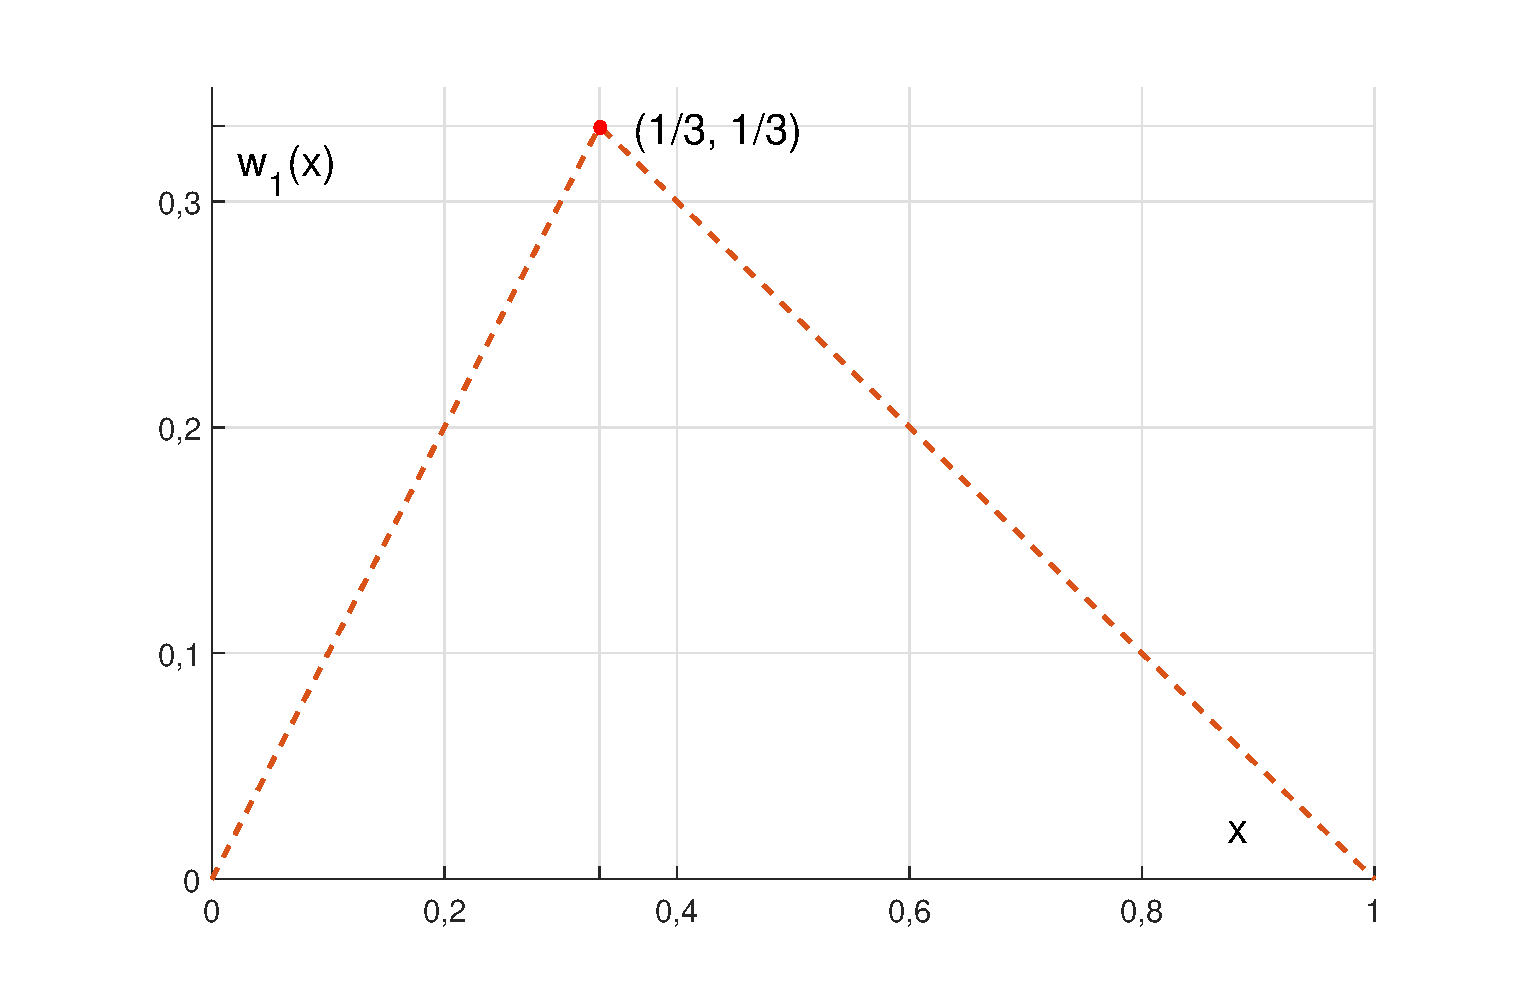
\includegraphics[width = 0.7\textwidth]{figP2OS.eps}
\caption{The payoff of player 1 as a function of $x$.}
\label{chap3:figP2OS}
\end{figure}


\end{example}
Contrary to general games in standard form, equilibria of 2POS games can be computed efficiently.  Indeed, remark that Player 1's problem, namely $$ \max{\min{ A \sigma_1}} ,$$ is simply an LP!  (In the above, $\sigma_1$ is the vector of his randomized stragegy profile, and $A$ is the payoff matrix.)
%\begin{figure}[!ht]
%\includegraphics[scale=1]{wip.png}
%\end{figure}


\ifx \globalmark \undefined %% This is default.
\bibliographystyle{plain}
\bibliography{../gametheorybibliography}
	\end{document}
\else 
	
\fi
